%%%%%%%%%%%%%%%%%%%%%%%%%%%%%%%%%%%%%%%%%%%%%%
%%%%%%%%%%   VORLAGE MASTERARBEIT   %%%%%%%%%%
%%%%%%%   Bruno Langbehn / TU BERLIN   %%%%%%%
%%%%%%%%%%%%%%%%%%%%%%%%%%%%%%%%%%%%%%%%%%%%%%


%%%%%%%%%%%%%   DEFINITIONEN   %%%%%%%%%%%%%%%

\documentclass[11pt,a4paper,twoside]{book}

%Packages
\usepackage[utf8]{inputenc}
\usepackage[german]{babel}
\usepackage[T1]{fontenc}
\usepackage{amsmath}
\usepackage{amsfonts}
\usepackage{amssymb}
\usepackage{graphicx}
\usepackage{xcolor}
\usepackage[textwidth=145mm,textheight=235mm,left=35mm,top=30mm,headsep=10mm]{geometry}
\usepackage{listings}
\usepackage{fancybox}
\usepackage[small,bf]{caption} %Schönere Beschriftungen für Abbildungen und Tabellen
\captionsetup{width=.9\textwidth,skip=5pt,format=plain,indention=5pt}
\usepackage{booktabs} %Schönere Tabellen
\usepackage{fancyhdr} %Schönere Kopfzeile
\usepackage[section,above]{placeins} %Abbildungen und Tabellen bleiben in ihrer Section
\usepackage{blindtext} %Einfügen von Blindtext über \blindtext
\usepackage{siunitx} %Einstellungen für Dezimaltrennzeichen und Definitionen in siunitx.cfg
\usepackage[autostyle=true,german=quotes]{csquotes} %Verwendung von Anführungszeichen über \enquote{Text}
\usepackage[titletoc]{appendix} %um eine Titelseite "Anhang" vor dem eigentlichen Anhang einfügen zu können

%Druckt den Hinweis "Entwurf" mit Datum auf jede Seite. Zum deaktivieren printwatermark=false setzen
\usepackage[printwatermark=true]{xwatermark}
\newwatermark[allpages,textcolor=gray!70,angle=0,xpos=68,ypos=-135,fontsize=14pt,fontfamily=phv]{Entwurf\ -\ \the\day.\the\month.\the\year}

\usepackage{hyperref} %pdf-Inhaltsverzeichnis und pdf-Links
\hypersetup{
pdfborder={0 0 0}, 
bookmarksnumbered=true,
pdftitle={Bachelorarbeit},
pdfauthor={Felix Frederik Zimmermann}
}

\setlength{\parindent}{0mm}

\newlength{\figwi}
\setlength{\figwi}{130mm}
\newlength{\fighi}
\setlength{\fighi}{100mm}
\newlength{\txtwi}
\setlength{\txtwi}{145mm}

%Tabellenabstände
\renewcommand{\textfraction}{0}
\renewcommand{\topfraction}{.75}
\renewcommand{\bottomfraction}{.75}
\renewcommand{\floatpagefraction}{.70}
\renewcommand{\arraystretch}{1.3}

%Appendices -> Anhang
\renewcommand*\appendixpagename{Anhang}
\renewcommand*\appendixtocname{Anhang}

%neue Pakete
\usepackage{verbatim} %kommentare
\usepackage[super,comma]{natbib} %bibliographie
%%%%%%%%%%%%%   MASTERARBEIT   %%%%%%%%%%%%%%%

\begin{document}

\pagestyle{plain}
\pagenumbering{Roman}


%%%%%%%%%%%%%%%   TITELSEITE   %%%%%%%%%%%%%%%

\begin{titlepage}
		
	\begin{center}
				
				
		\begin{flushright}
			\includegraphics[width=.3\textwidth]{images/TU_Logo.pdf}\\[2.5cm]    
			\end{flushright}
					
					
			{\newcommand{\HRule}{\rule{\linewidth}{0.5mm}}
				\HRule \\[0.4cm]
				\LARGE{\bfseries Simulation von Röntgenstreubildern\\ dreidimensionaler Nanostrukturen\\ für eine vergleichende Analyse von\\ Holographie und iterativer Phasenrekonstruktion}\\
							
				\HRule \\[1.5cm]}
			\textsc{\Large Bachelorarbeit}\\[0.5cm]
					
			\emph{vorgelegt von}\\
			Felix Frederik Zimmermann\\
			Matrikel-Nr. 343004\\[0.5cm]
			{\large \today}
					
					
			\vfill
					
			Technische Universität Berlin\\
			Fakultät II - Mathematik und Naturwissenschaften\\
			Institut für Optik und Atomare Physik\\
			Arbeitsgruppe Prof. Dr. Thomas Möller\\
					
		\end{center}
			
	\end{titlepage}
\clearpage
{\pagestyle{empty}\cleardoublepage}%


%%%%%%%%   SELBSTÄNDIGKEITSERKLÄRUNG   %%%%%%%

\begin{minipage}[b][12cm]{\textwidth}
\begin{center}
\begin{tabular}{c}

\textbf{Die selbständige und eigenhändige Anfertigung} \\
\textbf{versichere ich an Eides statt.} \\
\\
\\
\midrule
\textbf{Datum / Unterschrift} \\
\end{tabular}
\end{center}
\end{minipage}

%\cleardoublepage


%%%%%%%%%%%%%%%%   ABSTRACT   %%%%%%%%%%%%%%%%

\pdfbookmark[0]{Abstract}{abstract}
\begin{minipage}[t][120mm]{\textwidth}
\begin{Huge}
\textbf{Kurzfassung}\vspace{12mm}
\end{Huge}



\end{minipage}


\begin{minipage}[t][0mm]{\textwidth}
\begin{Huge}
\textbf{Abstract}\vspace{12mm}
\end{Huge}

\blindtext


\end{minipage}
%\cleardoublepage


%%%%%%%%%%%   INHALTSVERZEICHNIS   %%%%%%%%%%%


\setlength{\parskip}{3mm}
\tableofcontents
\cleardoublepage



%%%%%%%%%%%%%%%%   KAPITEL   %%%%%%%%%%%%%%%%%

\pagenumbering{arabic}
\pagestyle{headings}
\fancyhf{} 
\pagestyle{fancy} 
\fancyhead[LE,RO]{\sc\thepage} 
\fancyhead[LO]{\sc\nouppercase\rightmark} 
\fancyhead[RE]{\sc\nouppercase\leftmark}
\renewcommand{\headheight}{14pt}

\chapter{Einleitung}
Sowohl in der Clusterphysik, wie auch in Bereichen der Biologie und Medizin besitzt die Untersuchung von feinsten Strukturen mit Auflösungen im Nanometerbereich einen immer größeren Stellenwert. Bei der optischen Abbildung besteht eine Auflösungsbeschränkung aufgrund von Beugungserscheinungen in Abhängigkeit von der Wellenlänge (Abbe-Limit). Bei kürzeren Wellenlängen ist jedoch zum einen die Konstruktion von als Linsen geeigneten optischen Elementen durch die bei dieser Wellenlänge kaum vom Vakuum verschiedene Brechzahl der Materialien erschwert. Freie-Elektronen-Laser erzeugen kohärente Strahlung bei kurzen Wellenlängen mit hoher Brillianz und ermöglichen durch elastische Lichtstreuung die Aufnahme von sogenannten kohärenten Streubildern ohne die Verwendung von optischen Elementen zur Abbildung. Dieses Verfahren wird als \textit{Coherent Diffraction Imaging (CDI)} bezeichnet~\cite{schultz2013chapter7}.

\textit{CDI} erlaubt es, Einzelbildaufnahmen von Proben mit hoher räumlicher und definierter zeitlicher Auflösung durchzuführen. Insbesondere bei biologischen Proben ist es von Interesse, dass im Gegensatz zu anderen Verfahren (wie der Elektronenmikroskopie) durch die Verwendung von Injektoren, die einzelne Partikel der Probe in den Strahl einbringen, kein Träger für die Probe benötigt wird und auch keine Präparation der Probe von Nöten ist. Somit wird deren Struktur bis zur Abbildung nicht beeinträchtigt. Mit \textit{CDI} konnten bereits Aufnahmen von Viruspartikeln sowie Clusterproben angefertigt werden~\cite{seibert2011}. Jedoch geht bei der Aufnahme des Streubildes die Phase der gebeugten Welle verloren, die einen großen Teil der Informationen trägt. Dies wird als das Phasenproblem bezeichnet~\cite{shechtman2015}. Hierfür wurde kürzlich als Lösungsansatz die \textit{Freiflug-Holographie} entwickelt, bei der neben der Probe ein zusätzliches Referenzobjekt mit abgebildet wird und aus der Wechselwirkung der gestreuten Wellen der beiden Objekte Informationen gewonnen werden können. Weiterhin existieren verschiedene Algorithmen zur sogenannten  iterativen Phasenrekonstruktion.

Zum Vergleich dieser beiden Ansätze ist es zweckhaft, zunächst simulierte Streubilder einzusetzen, sodass die Ergebnisse der Rekonstruktion mit einem bekannten Ausgangsbild verglichen werden können. Es sind in der Literatur verschiedene Ansätze zur Simulation von Streubildern beschrieben, die gebräuchlichsten sind hierbei \textit{FDTD (Finite Difference Time Domain)}, \textit{DDA (Discrete Dipole Approximation)}, die 3D-Fouriertransformation ausgewertet auf der Ewaldkugel (berechnet mittels einer im Frequenzraum nicht äquidistanten schnellen Fouriertransformation) sowie sogenannte \textit{Multislice} Simulationen~\cite{drezek1999,sander2014,hantke2016,hare1994,barke2015}. Die erstgenannten Ansätze sind für die Simulation von Streubildern, wie sie für die Evaluation der Holographie benötigt werden, nur eingeschränkt geeignet, da bei der gewünschten hohen räumlichen Auflösung und der Ausdehnung der Objekte der Speicherbedarf das technisch Machbare um Größenordnungen überschreitet. Unter dem Begriff \textit{Multislice} hingegen werden verschiedene Ansätze subsumiert, die auf Näherungen aus der Wellenoptik aufbauen und die Menge an gleichzeitig zu bearbeitenden Daten durch eine schichtweise Formulierung des Problems reduzieren. 

Im Rahmen dieser Arbeit werden zunächst zwei verschiedene Formulierungen der schichtweisen Simulation des Durchtritts einer Wellenfront durch ein dreidimensionales Objekt sowie eine aus der Born-Näherung abgeleitete Simulation des Streubildes, die alle drei unter dem Begriff \textit{Multislice} beschrieben werden, betrachtet. Sie werden durch einen Vergleich mit der Mie-Streutheorie bewertet um die geeignetste Methode für die Simulation ausgedehnter Strukturen auszuwählen. Die beiden Ansätze zur Lösung des Phasenproblems, die Holographie sowie die iterative Phasenrekonstruktion werden anschließend zunächst für 2D Bilder verglichen, um im Anschluss die simulierte Austrittswelle hinter einer dreidimensionalen Nanostruktur aus dem simulierten Streubild zu rekonstruieren.
\chapter{Theoretischer Hintergrund}
\label{c_theorie}
 
\section{Skalare Beugungstheorie}

Aus den Maxwell-Gleichungen lässt sich unter der Annahme eines sich im Vergleich zur Wellenlänge $\lambda$ nur langsam ändernden Mediums die skalare Helmholzgleichung 
\begin{equation}
(\Delta+k^2\eta^2)\phi=0
\end{equation}
mit der Wellenzahl $k$
\begin{equation}
	k=\frac{2\pi}{\lambda}
\end{equation} und der komplexen Brechzahl des Mediums $\eta$ aufstellen. Diese Betrachtung ignoriert den vektoriellen Charakter der Elektrodynamik, insbesondere die Polarisation der Welle wird vernachlässigt. Des weiteren findet eine Separation der Zeitabhängigkeit statt, sodass nur stationäre Probleme betrachtet werden.

Im Bereich der Röntgenbeugung ist aufgrund der geringfügigen Abweichungen der Brechzahlen von Medien zur Vakuumbrechzahl ($\eta=1$) hilfreich $n\eta$ als
\begin{alignat}{2}
\label{eq:brechzahl}
	&\eta&&=1-\delta+i\beta=1 + \delta n \\
\label{eq:approxbrechzahl}
	&\eta^2&&\approx 1 + 2\delta n
\end{alignat}
darzustellen. Bei dieser Darstellung quantifiziert $\delta$ die Refraktion, $\beta$ die Absorption \cite[S. 21]{attwood1999}.

Die Fouriertransformation der Wellengleichung lautet mit der Näherung \ref{eq:approxbrechzahl} und unter Beachtung des Faltungstheorems
\begin{equation}
	(-q^2+k^2)\tilde{\phi}=\frac{-2k^2}{(2\pi)^{\sfrac{3}{2}}}(\tilde{\delta \eta} \ast \tilde{\phi})
\end{equation}
Wird nun die Greensche Funktion $\tilde{G}$ als
\begin{equation}
	\tilde{G}=\frac{1}{(2\pi)^{\sfrac{3}{2}}}\frac{2k^2}{q^2-k^2}
\end{equation}
definiert, so ist die inverse Fouriertransformation von $\tilde{G}$ divergent. Durch Hinzufügen von $\epsilon$ (mit $\epsilon\rightarrow 0^+$) im Nenner lässt sich die retardierte Greensche Funktion 


\begin{align}
G&=\int_{-\infty}^{\infty} \frac{2k^2}{q^2-k^2+0^+} e^{i\vec{q}\vec{r}}\dif^3 \vec{q}\nonumber\\
&\propto\frac{e^{iqr}}{r}
\end{align}
konstruieren \cite{trigg2006}. Für die Wellengleichung gilt somit im Fourier bzw. im Realraum \cite{cowley1995,thibault2007}:
\begin{align}
\tilde{\phi}&=\tilde{G}(\tilde{\delta \eta} \ast \tilde{\phi})\\
\phi&={G}\ast({\delta \eta}  {\phi})
\end{align}

\section{Born-Näherung}
Eine Ansatz für  eine Lösung der Wellengleichung lässt sich in Form einer Reihe
\begin{equation}
\phi=\phi_0+\phi_1+\phi_2+..
\end{equation}
(mit $\phi_0$ als einlaufende Welle) aufstellen. Ist die Amplitude der gestreuten Welle deutlich geringer als die der einfallenden Welle, so lässt sich in XX die Näherung $\phi\approx\phi_0$ im mit $G$ zu faltenden Term anwenden. Dies wird als Born Näherung erster Ordnung bezeichnet. Somit gilt für die Lösung der Wellengleichung

\begin{equation}
\phi\approx\phi_0+G\ast({\delta \eta} \phi_0)
\end{equation}
Ist die einfallende Welle eine ebene Welle $\phi_0=e^{ik_0r}$ und wird der Betrachtungsabstand als groß gegenüber XXX angenommen, so lässt mit der Näherung

\begin{equation}
|r-r'|=\sqrt{r^2+r'-2rr'}\approx r-\frac{\vec{r'}\vec{r}}{r}=r-\frac{\vec{k}}{k_0}\vec{r'}\approx r
\end{equation}
für die gestreute Welle mit dem Streuvektor $\vec{q}$ ($\vec{k}=\vec{k_0}+\vec{q}$)
\begin{equation}
\int G(\vec{r}-\vec{r}')\delta\eta(\vec{r}') exp^{ik_0r'}  \dif \vec{r}'\approx e^{ik_0r}\int \delta\eta(\vec{r}')e^{-i\vec{q}\vec{r}'}\dif \vec{r}'\propto \mathscr{F}[\delta\eta]
\end{equation}
aufstellen. Somit ist in dieser Näherung die gestreute Welle proportional zur dreidimensional fouriertransformierten Abweichung der Brechzahl von der Vakuumbrechzahl.




\section{Angular-Spectrum Propagation}
Wird eine elektromagnetische Welle $\phi$ durch ihre zweidimensionale Fouriertransformierte $\bar{\phi}$ als
\begin{equation}
\phi(x,y,z)=\frac{1}{\sqrt{2\pi}}\iint_{-\infty}^{\infty}\bar{\phi}(f_x,f_y,z)e^{i(q_xx+q_yy)} \dif q_x \dif q_y
\end{equation}dargestellt und gefordert dass diese im Vakuum die Wellengleichung XXX erfüllt,
so muss $\bar{\phi}$
\begin{equation}
	\frac{\partial ^2}{\partial z^2}\bar{\phi}(q_x,q_y,z)^2+ \left(k^2-\left(q_x+q_y\right)\right)\bar{\phi}(q_x,q_y,z)=0
\end{equation}
erfüllen. Eine Lösung dieser Gleichung ist
\begin{equation}
\bar{\phi}\left(q_x,q_y,\Delta z\right)=\bar{\phi}(q_x,q_y,0)e^{i\Delta z\sqrt{k^2-(q_x+q_y)^2}}\, . 
\end{equation}
Somit lässt sich die Propagation einer Welle im Vakuum als Multiplikation mit einem Exponentialfaktor im Fourierraum beschreiben. Dieses Verfahren wird \textit{Angular-Spectrum} Propagation genannt \cite{goodman2005}. 
Die eingehende Welle bei $z=0$ wird hierbei in ebene Wellen, die sich in verschiedene Richtungen ausbreiten (Angular Spectrum) zerlegt und deren Propagation berechnet. Die ausgehende Welle bei $z=\Delta z$ lässt sich aus $\bar{\phi}\left(q_x,q_y,\Delta z\right)$ durch eine inverse Fouriertransformation bestimmen.



\section{Fresnel- und Fraunhofer-Näherung}
Wird in XXXFormel die Taylor-Näherung 2. Ordnung
\begin{equation}
	\sqrt{k^2-(q_x+q_y)^2}\approx k-\frac{(q_x^2+q_y^2)}{2k}
\end{equation}
durchgeführt und eine zweidimensionale inverse Fouriertransformation angewendet, so erhält man mit dem Faltungstheorem die Fresnel-Näherung 

\begin{align}
\bar{\phi}(x,y, z)&=\bar{\phi}(x,y,0) e^{ik z}e^{\frac{i z}{2k}(q_x^2+q_y^2)}\\
\phi(x,y, z)&=\phi(x,y,0) \ast \left(
\frac{e^{ik z}}{i z \lambda } 
e^{ik\frac{(x^2+y^2)}{2 z}}
\right)
\end{align}
In dieser Näherung wird die Ausbreitung der Welle durch die Faltung dem sogenannten Fresnel-Propagator ausgedrückt. Wird die Faltung explizit ausgeschrieben, kann der Exponent aufgespalten werden


\begin{align}
\phi(x,y, z)&=\frac{e^{ikz}}{iz\lambda}
\int_{-\infty}^\infty 
\phi(\alpha,\beta,0)
e^{\frac{ik}{2z}\left(\left(x-\alpha\right)^2+\left(y-\beta\right)^2\right)}
\dif \alpha \dif \beta \nonumber \\
&=\frac{e^{ikz}}{iz\lambda}e^{\frac{ik}{2z}(x^2+y^2)}
\int_{-\infty}^\infty 
\phi(\alpha,\beta,0)
e^{\frac{ik}{2z}\left(\alpha^2+\beta^2\right)}
e^{\frac{-ik}{ z}\left(x\alpha+y\beta\right)}
\dif \alpha \dif \beta
\end{align}



Verschwindet die eingehende Welle $\phi_(x,y,0)$ außerhalb eines Bereiches $S=[-X,X]\times[-Y,Y]$ und gilt 
\begin{equation}
\forall \alpha,\beta \in S:	z\gg \frac{k}{2}\left(\alpha^2+\beta^2\right) \, , 
\end{equation}
d.h. sind die Ausmaße des Bereiches, auf dem die Welle nicht verschwindet klein gegenüber dem Beobachtungsabstand, so gilt
\begin{equation}
e^{\frac{ik}{2z}\left(\alpha^2+\beta^2\right)}\approx 1
\end{equation}
und Gleichung XXX lässt sich als Fouriertransformation der Eingangswelle ausgewertet bei $f_{x,y}=\tfrac{k}{z}(x,y)$ und multipliziert mit einem in $x,y$-Richtung reinem Phasenterm interpretieren:

\begin{equation}
\phi(x,y)=\frac{e^{ik(z+\frac{x^2+y^2}{2z})}}{iz\lambda}\mathscr{F}\left[\phi_(x,y,0)\right](f_x=\tfrac{kx}{z},f_y=\tfrac{kx}{z}) \, ,
\end{equation}
Diese Näherung wird als Fraunhofer-Näherung bezeichnet.

\begin{comment}

\subsubsection{Subsubsection}

\paragraph{Paragraph}



\section{Abbildungen}
Eine Beispiel-Abbildung ist in Abb. \ref{Abb:BspAbbildung} gezeigt.

\begin{figure}
\centering
\includegraphics[width=0.9\textwidth]{images/SchemaErzeugungNachweis.jpg}
\caption[Abbildungstext im Abbildungsverzeichnis]{Abbildungsunterschrift. Abbildung nach \cite{B-SViel}.}
\label{Abb:BspAbbildung}
\end{figure} 



\section{Tabellen}
Eine Vorlage ist in Tabelle \ref{Tab:BspTabelle} gegeben.
 
\begin{table}
\centering
\begin{tabular}{SccrrS}
\hline\hline
{Druck [\si{\milli\bar}]} & Gas &  $T_0$ [K]& $\Gamma^\ast$ & $\langle N \rangle$ & {$R$ [nm]}\\
\hline
1000 & Ar &  300 & 2.325 & 240 & 1,3\\
1000 & Ar &  300 & 2.971 & 426 & 1,6\\
1000 & Xe &  300 & 7.845 & 4.177 & 3,9\\
1000 & Xe &  300 & 10.024 & 6.337 & 4,4\\
\hline
5000 & Ar &  300 & 11.625 & 8.274 & 4,2\\
5000 & Ar &  300 & 14.854 & 12.862 & 4,9\\
5000 & Xe &  300 & 39.226 & 73.863 & 10,1\\
5000 & Xe &  300 & 50.121 & 114.826 & 11,7\\
\hline
10000 & Ar & 300 & 23.250 & 28.812 & 6,3\\
10000 & Ar & 300 & 29.708 & 44.790 & 7,4\\
10000 & Xe & 300 & 78.452 & 257.207 & 15,3\\
10000 & Xe & 300 & 100.243 & 399.848 & 17,7\\
\hline
8000 & Xe &  220 & 127.589 & 617.258 & 20,4\\
8000 & Xe &  220 & 163.029 & 959.574 & 23,7\\
\hline\hline
\end{tabular}
\caption[Text für Tabellenverzeichnis]{Tabellenunterschrift.}
\label{Tab:BspTabelle}
\end{table}

\section{Anführungszeichen}
Anführungszeichen werden global über das Paket \emph{csquotes} gesetzt und wie folgt eingebunden:

\verb+\enquote{Text in Anführungszeichen}+

Ausgabe: \enquote{Text in Anführungszeichen}.



\section{Setzen von Einheiten}
Zum Setzen von Einheiten wird das Package \emph{siunitx} verwendet:

Zahlen: \num{83567}, \num{,23e-16}, \num{3,89+-0,03}

Winkel: \ang{12.3}, \ang{1;2;3}

Wert mit Einheit: $v_{max}=\SI{260}{\m/\s}$, $v_\infty=\SI{173}{\metre\per\second}$, $R = \SI[per-mode=symbol]{8,3144621}{\joule\per\mol\per\kelvin}$

Wert mit Fehler und Einheit: $T_0=\SI{5,234(15)}{\kelvin}$

Celsius: $T_S=\SI{38.6}{\celsius}$ 

Minuten: $t_c=\SI{90}{\min}$

Druck: $p_0=\SI{80}{\bar}$, Hintergrunddruck \SI{1,9e-9}{\torr}


 
\subsection{Einheiten in Tabellen}
Die Verwendung von Einheiten in Tabellen mit dem Paket \emph{siunitx} ist in Tabelle \ref{Tab:BspS} gezeigt.
\begin{table}
\centering
\begin{tabular}{lSSSSS}
\hline\hline
 & {He} &  {Ne} & {Ar} & {Kr} & {Xe}\\
\hline
$\Gamma_{ch}$ [\SI{e16}{\metre\tothe{\num{-2.15}}\kelvin\tothe{\num{-1.2875}}}] & 36,189 & 31,07 & 3,495 & 1,9531 & 231,036\\
$K_{ch}$ [\si{\K\tothe{\num{2.2875}}\per\milli\bar\micro\metre\tothe{\num{0.85}}}] & 34,865 & 18,5 & 16,46 & 2980,982 & 5,554\\
\hline\hline
\end{tabular}
\caption[Beispiel für die \emph{siunitx}-Klasse \enquote{S} in Tabellen]{Mit der Klasse \enquote{S} des \emph{siunitx}-Pakets werden Zahlen in Tabellen am Dezimaltrennzeichen ausgerichtet. Normaler Text muss dann in geschweiften Klammern gesetzt werden.}
\label{Tab:BspS}
\end{table}


\section{Blindtext}
\end{comment}

\chapter{Problemstellung}

..phasenproblem..
.. bewertung schwierig bei unbekanntem eingangssignal

Somit ergibt sich als Problemstellung dieser Arbeit erstens die Erzeugung von simulierten Streubildern sowie deren Verifizierung.
Im zweiten Schritt werden an 2D-Bildern die Eigenschaften der zu verwendenden Rekonstruktionsansätze betrachtet um schließlich die zuvor erstellten Referenzbilder rekonstruieren zu können.

\chapter{Simulation von Streubildern}
Das Problem der Berechnung synthetischer Streubilder besitzt verschiedene Lösungsansätze..
\section{Mie Streuung}
Die Mie-Theorie bietet eine analytische Lösung der Streuung an einer Kugel  in Form einer unendlichen Reihe, die numerisch ausgewertet werden kann \cite{bohren2008}. Für die Intensität beim Streuwinkel $\theta$ gilt in dieser Theorie für die Streuung unpolarisierter Strahlung in Abhängigkeit von der Brechzahl $\eta$ der Sphäre (Radius $r$) und dem Parameter $x=r/k$:
\begin{equation}
I(\theta)\propto\frac{1}{2}\left(\abs{S_1}^2+\abs{S_2}^2\right)
\end{equation} 
mit
\begin{align}
S_1=\sum_j{\frac{2n+1}{n(n+1)}(a_n\pi_n+b_n\tau_n)} &&S_2=\sum_n{\frac{2n+1}{n(n+1)}(a_n\tau_n+b_n\pi_n)}
\end{align}
wobei die Reihe bei der numerischen Auswertung nach $N$ Termen abgebrochen wird. Eine hinreichende Konvergenz liegt meist bei $N\approx2+x+4\sqrt[3]{x}$ Termen vor.  $\pi_n$ und $\tau_n$ können mit $\pi_1=1$ und  $\pi_2=3\cos{\theta}$ rekursiv über die Relationen
\begin{align}
&\pi_n=\frac{2n-1}{n-1}\cos{\theta}\pi_{n-1}-\frac{n}{n-1}\pi_{n-2}&&\tau_n=n\cos{\theta}\pi_n-(n+1)\pi_{n-1}\\
\end{align}
und $a_n$,$b_n$ über 
\begin{align}
a_n=\frac{(D_n/\eta+n/x)\psi_n-\psi_{n-1}}{(D_n/\eta+n/x)\chi_n-\chi_{n-1}} &&
b_n=\frac{(\eta D_n+n/x)\psi_n-\psi_{n-1}}{(\eta D_n+n/x)\chi_n-\chi_{n-1}}
\end{align} definiert werden. $D_n$ lässt sich rekursiv über
\begin{align}
D_{N+15}=0 && D_{n-1}=\frac{n}{\eta*x}-\frac{1}{D_n+n/(\eta x)}
\end{align}
und $\psi_n$,$\chi_n$ mittels sphärischer Besselfunktionen 1. Art ($j_n$) und 2. Art ($y_n$) als 
\begin{align}
\psi_n=x j_n&&  \chi_n=x j_n+ixy_n
\end{align}
berechnen \cite[S. 112f, 95, 127f]{bohren2008}.
Eine vektorisierte Version dieser Berechnung liegt in der auf Mätzler \cite{maetzler2002} basierten Matlab Funktion \texttt{simulation/mie.m} vor und dient der Verifizierung der Simulationsverfahren.

\section{Projektion}
	Näherung der dreidimensionalen Streuobjekte durch zweidimensionale Blenden durch Projektion. Für diese Projektionen lässt sich in Fraunhofer-Fernfeldnäherung das Streubild darstellen XXX. 
	
	Für eine kreisförmige Blende exisistiert eine analytische Darstellung der Fouriertransformation in Form der sogenannten Airy-Scheibe und das Streubild lässt sich somit mittels der Besselfunktion 1. Ordnung $J_n$ als
	\begin{equation}
	I(\theta) \propto \left ( \frac{2 J_1(kr \sin \theta)}{kr \sin \theta} \right )^2 
	\end{equation}
	berechnen\cite[S. 396]{born1980}. Für nicht kreisförmige Projektionen der Dichte lässt sich die Fouriertransformation diskret numerisch auswerten.
	Eine weitere gebräuchliche Näherung für kugelförmige Objekte ist die Rayleigh-Gans Näherung (gültig für kleine Radien und Brechzahlen nahe Vakuum). In dieser nimmt die Intensität die Form
	\begin{equation}
	    I(\theta)\propto\left ( \frac{j_1(2kr\sin(\theta/2))}{2kr\sin(\theta/2)} \right )^2 
	\end{equation}
	mit der sphärischen Besselfunktion $j_n$ an \cite[S. 163]{bohren2008}. 


\section{Multislice Fourier Transformation}
	Nach XX gilt in der ersten Bornschen Näherung für die Amplitude der gestreuten Welle
	\begin{equation}
		\phi\propto\int \delta\eta(\vec{r}) e^{-i\vec{q}\cdot \vec{r}} \dif \vec{r}
	\end{equation}
	mit $\vec{r}=(x,y,z)^T$ und  $\vec{q}=(q_x,q_y,q_z)^T$. Wird das Skalarprodukt $\vec{q}\cdot \vec{r}=xq_x+yq_yzq_z$ ausgeschrieben und die Integration über $x$ und $y$ als zweidimensionale Fouriertransformation interpretiert
	\begin{equation}
	\phi\propto\int \mathscr{F}\left[\delta\eta\right](q_x,q_y,z) e^{-zq_z} \dif z \, ,
	\end{equation}

	so lässt sich das Integral in z-Richtung als Summe interpretieren sofern sich $q_z$ als $q_z=q_\parallel(q_\perp)$ ausdrücken lässt.
	Aufgrund der Impulserhaltung muss $k_{ein}^2=k_{aus}^2=k^2$ gelten. Nach Abbildung XXX 
	\begin{align}
	k^2=(k-q_\parallel)^2+q_{\perp}^2
	\Leftrightarrow q_\parallel=k-\sqrt{k^2-q_\perp^2}
	\end{align}
	\begin{equation}
	\phi\approx\sum_n{\mathscr{F}\left[\rho_z\right] e^{-in\delta_z\left(k-\sqrt{k^2-q_\perp^2}\right) }}
	\end{equation}

	\begin{figure}
		\centering
		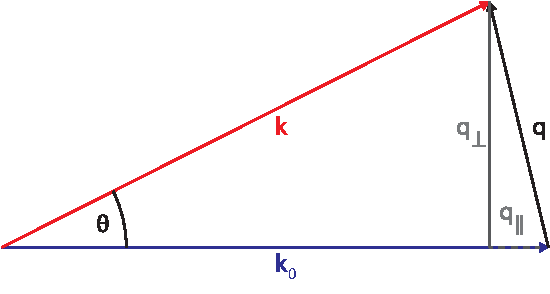
\includegraphics[width=0.5\textwidth]{images/msft.eps}
		\caption[Abbildungstext im Abbildungsverzeichnis]{Skizze zur Bezeichnung der Vektoren. $k_{ein}$ und $k_{aus}$ bezeichnen den Wellenvektor der einfallenden bzw. ausfallenden Welle mit dem dazwischenliegenden Winkel $\theta$. $q$ bezeichnet den Streuvektor mit einer zu $k_{ein}$ parallelen ($q_{||}$) und einer senkrechten ($q_\perp$) Komponente.. }
		\label{Abb:BspAbbildung}
	\end{figure} 

	Formel XXX beschreibt einen Algorithmus um das Streubild eines dreidimensionalen Objektes im Fernfeld in der 1. Bornschen Näherung zu berechnen. Diese Methode wird als Multislice Fourier Transformation (MSFT) bezeichnet \cite{barke2015}. Bei dieser wird Mehrfachstreuung ignoriert. Durch nachträgliches Einführen eines zusätzlichen Faktors XXX der die Absorption und Phasenänderung der Welle beim Durchlaufen des Objektes beschreibt, lässt eine grobe Näherung für Absorptionseffekte einzuführen. Eine Implementation des MSFT-Algorithmus liegt in \texttt{simulation/msft.m} vor 

\section{Multislice Propagation}
	Ein alternatives Verfahren zur Simulation XX ist in der Literatur als Multislice oder Beam Propagation bekannt \cite{hare1994}\cite{cowley1957}. Dieses Verfahren basiert auf ...
	Die Szene, deren Streubild zu berechnen ist, wird in einzelne Schichten zerlegt.
	Die Ausbreitung der in Szene einfallende ebene Welle wird genähert durch eine Vakuumpropagation von Schicht zu Schicht nach Angular Spectrum Propagation
	\begin{equation}
\bar{\phi}\left(z+\Delta z\right)=\bar{\phi}(z)e^{i\Delta z\sqrt{k^2-(q_x+q_y)^2}}\, . 	\Phi(z+\Delta z)=
	\end{equation}
	sowie eine Wechselwirkung mit der Materie der Schicht in einer einzelnen Ebene
	\begin{equation}
		\phi(z+\Delta z)=\phi e^{i\delta n \Delta z}
	\end{equation}.
	
	\begin{figure}
		\centering
		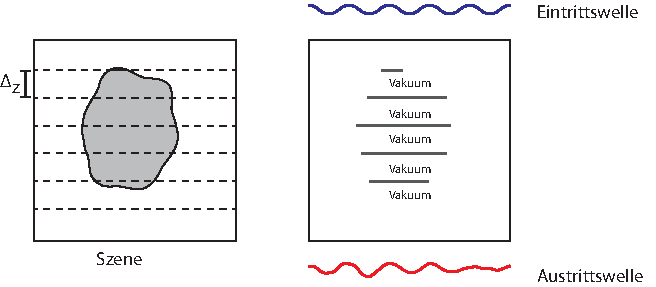
\includegraphics[width=0.75\textwidth]{images/multislice.eps}
		\caption[Abbildungstext im Abbildungsverzeichnis]{Prinzip Multislice Propagation. Die Szene wird in einzelne Schichten zerlegt und die Wechselwirkung mit der Materie jeder einzelnen Schicht in auf eine in dieser Schicht liegenden Ebene reduziert. Zwischen diesen Ebenen wird eine Vakuumpropagation angewendet.}
		\label{Abb:BspAbbildung}
	\end{figure} 
	
	(Die Näherung der Vakuumausbreitung durch einen Fresnel-Propagator bringt gegenüber der korrekten Berechnung über die Angular Spectrum Propagation keine numerischen Vorteile. Aus diesem Grund wird im Gegensatz zu \cite{hare}XXX auf diese Näherung verzichtet). 
	Bei diesem Verfahren wird die Annahme getroffen, dass  innerhalb einer Schicht die örtliche Verteilung der Materie konstant ist, sowie die durch die Propagation bedingte ... vernachlässigbar ist\cite{hare1994}. Des Weiteren wird bei der wird bei der Wechselwirkung mit der Materie der Winkel vernachlässigt XXX.
	
	Der Algorithmus zur Berechnung der Austrittswelle lautet somit
	\begin{equation}
\Phi(z+\Delta z)=
	\end{equation}
	Ist die Austrittswelle bekannt, so ist die weitere ausbreitung zum Detektor eine Vakuumpropagation, die sich entweder mittels Angular Spectrum Propagation berechnen lässt, oder sich durch eine einfache Fouriertransformation in Fraunhofer-Näherung bestimmen lässt. Ersteres Verfahren hat den Nachteil, das es bei einer numerischen Implemantion im Bereich der Szene die gleiche räumliche Rastergröße wie im Bereich des Detektors erfordert, während bei Anwendung der Fernfeld Näherung xxx
\section{Thibaults Multislice}
Thibault stellt in XX einen eigene Formulierung der Multislice-Simulation auf. Ausgehend von der Wellengleichung XX
lässt sich für die Austrittswelle XXX aufstellen.
\begin{equation}
\tilde{\Phi}(z)=\tilde{G}\ast_z\left[\tilde{\delta\eta}\ast_{q_\perp} \tilde{\Phi}\right]
\end{equation}
\begin{equation}
\tilde{G}=\frac{1}{2\pi}\frac{ik^2}{\sqrt{k^2-q_\perp^2}}e^{iz(\kappa-k)}
\end{equation}
unter der Vernachlässigung von Rückstreuung lässt sich das Faltungsintegral als in zwei Integrationsbereiche aufspalten
\begin{equation}
\tilde{\Phi}(z+\Delta z)=
\int_{\Delta z}^{\infty} \tilde{G}(z')\left[\tilde{\delta\eta}\ast_{q_\perp} \tilde{\Phi}\right](z+\Delta z-z')\dif z'
+
\int_{0}^{\Delta z} \tilde{G}(z')\left[\tilde{\delta\eta}\ast_{q_\perp} \tilde{\Phi}\right](z+\Delta z-z')\dif z'
\end{equation}
Für den ersten Summanden gilt

\begin{align*}
&\stackrel{\hphantom{z'\rightarrow z''+\Delta z}}{\hphantom{=}} 
\int_{\Delta z}^{\infty} \tilde{G}(z')\left[\tilde{\delta\eta}\ast_{q_\perp} \tilde{\Phi}\right](z+\Delta z-z')\dif z'\\
&\stackrel{z'\rightarrow z''+\Delta z}{=}
\int_{0}^{\infty} \tilde{G}(z''+\Delta z)\left[\tilde{\delta\eta}\ast_{q_\perp} \tilde{\Phi}\right](z-z'')\dif z''\\
&\stackrel{\hphantom{z'\rightarrow z''+\Delta z}}{=}
e^{i\Delta z(\kappa-k)}\int_{0}^{\infty} \frac{1}{2\pi}\frac{ik^2}{\sqrt{k^2-q^2_\perp}}e^{iz''(\kappa-k)}\left[\tilde{\delta\eta}\ast_{q_\perp} \tilde{\Phi}\right](z-z'')\dif z''\\
&\stackrel{\hphantom{z'\rightarrow z''+\Delta z}}{=}
e^{i\Delta z(\kappa-k)}\tilde{\Phi}(z) \numberthis
\end{align*}
Im zweiten Summanden kann für hinreichend kleine $\Delta z$ das Integral gut durch eine Rieman-Obersumme mit einem einzigen Stützpunkt approximiert werden:
\begin{equation}
\int_{0}^{\Delta z} \tilde{G}(z')\left[\tilde{\delta\eta}\ast_{q_\perp} \tilde{\Phi}\right](z+\Delta z-z')\dif z'
\approx
\Delta z \tilde{G}(\Delta z)\left[\tilde{\delta\eta}\ast_{q_\perp} \tilde{\Phi}\right](z)
\end{equation}
Für den Fehler 
\begin{equation}
\text{Rieman Abschätzung}
\end{equation}
Somit lässt sich in Näherung für die Welle bei $z+\Delta z$
\begin{equation}
\tilde{\Phi}(z+\Delta z)
\approx
e^{i\Delta z(\kappa-k)}
\left[
\tilde{\Phi}(z)+\frac{\Delta z}{2\pi}\frac{ik^2}{\sqrt{k^2-q^2_\perp}}
\right]
\end{equation}
Die numerische Simulation dieser Methode ist in \texttt{simulation/thibault.m} implementiert.


\section{Ergebnisse und Diskussion}
\subsection{Verifizierung}
Zur Verifizierung der vorgestellten Simulationsalgorithmen und deren numerische Implementierungen eignet sich der Vergleich der berechneten Streubilder hinter Kugeln mit den Ergebnissen aus der Berechnung mittels Mie-Streuung. Der vergleich wird für verschiedene Brechzahlen, Kugelradien und Berechnungsauflösungen bei einer Wellenlänge von 1\si{nm} durchgeführt.
Zur Quantifizierung des Vergleichs wird die Summe der Betragsquadrat der Abweichung zwischen den Simulationsdatenpunkten und der Berechnung mittels Mie verwendet.


XXWelche Paramerter?
hier Bild von Austrittswellen und Streubilder
Radialprofile
Plot der Fehler

Zur Quantifizierung der Genauigkeit der Simulationen wird die Summe der quadratischen Abweichungen der Datenpunkte der aus den Streubildern erzeugten Radialprofile von der Mie-Lösung betrachtet:


\subsection{Austrittswellen}
darstellung von interessanten austrittswellen von mehreren objekten und vgl. mit summe aus einzel austrittswellen
\chapter{Rekonstruktion}
Nach XX entspricht die im Fernfeld aufgenommene Welle der Fouriertransformierten der Austrittswelle. Könnte sowohl Amplitude als auch Phase aufgenommen werden, so ließe sich durch eine einfache Rücktransformation die Austrittswelle rekonstruieren und somit Informationen über das Objekt gewinnen. Jedoch wird mittels eines Sensors nur die Amplitude der Welle aufgezeichnet, die Informationen über die Phase gehen somit verloren. Das Problem, aus dieser unvollständigen Messung die Austrittswelle zu rekonstruieren wird als das Phasenproblem bezeichnet. Zur Lösung existiert u.A. der Ansatz der Freiflug-Holographie sowie die Methode der iterativen Phasenrekonstruktion
\section{Holographie}
Angenommen neben dem Objekt, über das Informationen gewonnen werden sollen befindet sich ein weiteres (im Weiteren als Referenz bezeichnetes) Objekt im Strahl, sodass die eingehende Welle an beiden gestreut wird. ...
\subsection{Auto- und Kreuzkorrelation}
\begin{equation}
	\mathscr{F}^{-1}\left[\left|\tilde{O}+\tilde{R}\right|^2\right]=
	\mathscr{F}^{-1}\left[\tilde{O}\tilde{O}^*\right]+
	\mathscr{F}^{-1}\left[\tilde{R}\tilde{R}^*\right]+
	\mathscr{F}^{-1}\left[\tilde{R}\tilde{O}^*\right]+
		\mathscr{F}^{-1}\left[\tilde{O}\tilde{R}^*\right]
\end{equation}
aus betragsquadrat wird korrelation 
\subsection{Entfaltung}
Die Kreuzkorrelation aus Objekt und Referenz entspricht einer Faltung des Objektes mit der gespiegelten, komplex konjugierten Referenz. Um eine bessere Approximation des Objektes zu erhalten, muss diese Faltung rückgängig gemacht werden. Nach Formel XXX entspricht die Faltung einer Multiplikation, die Inverse somit einer Division im Fourierraum. Jedoch verursachen sowohl Rauschen wie auch Singulariäten in der fouriertransformierten Referenz Probleme.

Das Problem der Entfaltung tritt in verschiedenen Bereichen auf, unter anderem in der Bildverarbeitung.
Hier ist der Prozess der Wiener Entfaltung etabliert. 



\section{iterative Phasenrückgewinnung}
Ist neben der Amplitude die Phase der Fouriertransformation der Austrittswelle bekannt, so kann diese durch eine inverse Transformation wiederhergestellt werden. 
Da bei N komplexen Datenpunkten im Realraum die Fouriertransformation durch N Amplituden und N Phasen, also 2N Variablen dargestellt werden kann, jedoch nur N Variablen (die Fourieramplituden) gemessen werden können ist das Problem unterbestimmt und nicht lösbar. Kann jedoch das zu rekonstruierende Objekt im Realraum auf N/2 Bildpunkte beschränkt werden, so wird das Problem lösbar. Die räumliche Beschränkung im Realraum wird 
durch die Wahl eines sog. Supports, außerhalb dessen der Realraum als leer angenommen wird umgesetzt.  
\subsection{Algorithmen}
kurze einführung der projektoren schreibweise, konkrete projektoren zu den algorithmen im anhang

Die Problemstellung ist eine Lösung der Gleichung $\rho(x)=\mathscr{F}^{-1}\tilde{\rho}(q)$ unter den Nebenbedingungen dass 1. $\rho$ auf den Support beschränkt ist und 2. die Amplituden von $\tilde{\rho}$ mit den bekannten Fourieramplituden $A(q)$ übereinstimmt.

Ein hierfür verwendeter Algorithmus, der Error-Reduction Algorithmus (ER) basiert auf abwechselnden Erzwingen der der Nebenbedingungen, d.h. von einem Startwert $\rho_0$ ausgehend wird zunächst $\tilde{\rho_0}$ bestimmt, die Amplitude im Fourierraum durch $A$ ersetzt, in den Realraum transformiert und dort außerhalb des Supports gleich Null gesetzt. Dies wird iterativ wiederholt, wobei sich $\rho_n$ einer beide Nebenbedingungen erfüllenden Lösung annähert.

Das Erzwingen der Nebenbedinung im Realraum kann als Projektion auf die Lösungsmenge $S$ der Nebenbedingung  mit dem Komplement $\bar{S}$ durch den Projektor $P_s$ 

 \begin{align}
 P_s\rho (x)=\begin{cases}
 \rho (x)  &\text{für } x\in S\\
 \mathbb{0}  &\text{für }x\notin S
 \end{cases}&&
 P_{\bar{s}}\rho (x)=\begin{cases}
 \mathbb{0} &\text{für } x\in S\\
 \rho (x)   &\text{für }x\notin S
 \end{cases}
 \end{align}
aufgefasst werden. Der analoge Projektor für die Erfüllung der Nebenbedingung im Fourierraum, der im Fourierraum die Amplitude von $\tilde{\rho}$ durch die bekannte Amplitude $A(q)$ ersetzt und dabei den Winkel $\Phi(q)$ beibehält lautet
\begin{align}
	\tilde{P}_m \bar{\rho}(q)&=A(q)e^{i\Phi(q)} &&P_m\rho(q)=\mathscr{F}^{-1}A(q)e^{i\Phi(q)}\mathscr{F}\rho(x)
\end{align}

	\begin{figure}
		\centering
		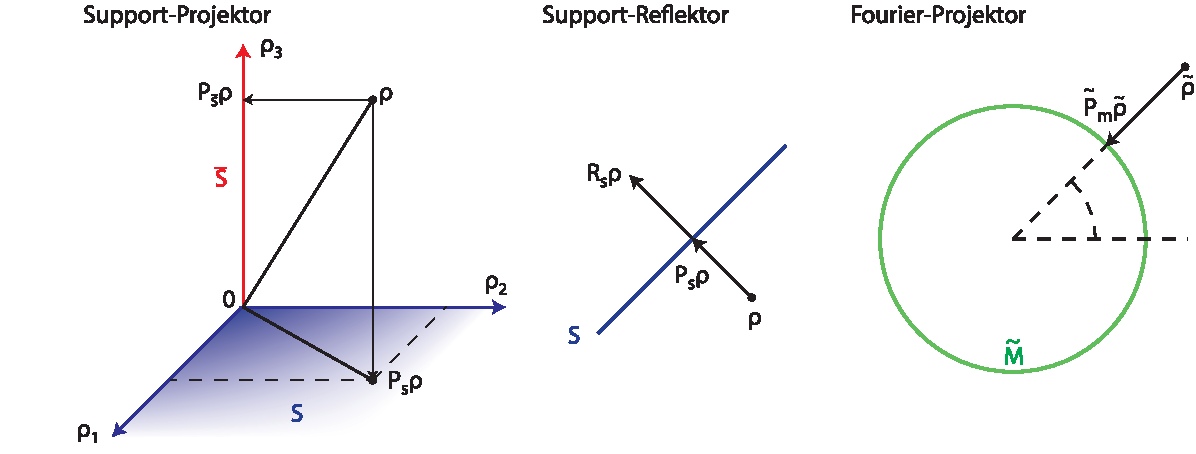
\includegraphics[width=0.75\textwidth]{images/projektor.eps}
		\caption[Abbildungstext im Abbildungsverzeichnis]{Abbildungsunterschrift. Abbildung nach \cite{B-SViel}.}
		\label{Abb:BspAbbildung}
	\end{figure}.
	Neben den Projektoren die, den Schritt $\rho\rightarrow (\mathbb{1}+(P-\mathbb{1}))\rho$ ausführen, können auch sogenannte Reflektoren mit doppelter Schrittweite
	\begin{equation}
	R_\nu= (\mathbb{1}+2(P-\mathbb{1}))=(2P_\nu-\mathbb{1})
	\end{equation}
	eingeführt werden.
In dieser Schreibweise können auch Weiterentwicklungen wie der Hybrid Input Output (HIO) und Relaxed Averaged Alternating Reflections (RAAR) Algorithmus dargestellt werden XXTabelleXX. Ihre Prinzip ist in XXX graphisch dargestellt.
	\begin{figure}
		\centering
		\includegraphics[width=0.75\textwidth]{images/algorithmen.eps}
		\caption[Abbildungstext im Abbildungsverzeichnis]{Abbildungsunterschrift. Abbildung nach \cite{B-SViel}.}
		\label{Abb:BspAbbildung}
	\end{figure} 
\subsection{Support}
Üblicherweise ist der Bereich auf den das Objekt im Realraum beschränkt ist nicht bekannt, der für die iterativen Rekonstruktionsalgorithmen benötigten Supports muss zunächst bestimmt werden. Hierfür existieren verschiedene Möglichkeiten. Die triviale Methode besteht aus einer Festlegung aus zuvor bekannten Dimensionen des Experiments. Jedoch kann nur in Ausnahmefällen so der Support ausreichend eng gewählt werden um die Bedingung XXX zur erfüllen.
Eine verbreitete Methode, bezeichnet als Shrink-Wrap Algorithmus, ist durch eine Anpassung des Supports während der Rekonstruktion gekennzeichnet: Der zunächst geratene (für eine eindeutige Lösung des Problems  zu große) Support wird nach einer festgelegten Anzahl an Rekonstruktionsiterationen auf den Bereich beschränkt, in dem die Rekonstruierte Intensität höher als ein festgelegter Schwellwert ist. Dieser aktualisierte Support wird für weitere Iterationen genutzt und erneut aktualisiert\cite{marchesini2003}.

Eine Zusammenführung der Holographie und der IPR 

Die aus der Holographie gewonnene Rekonstruktion des Objektes und eine Schätzung der Referenz lassen sich zu einem Support kombinieren. Der nötige Abstandsvektor dieser Supportteile ist der  Abstandsvektor zwischen Auto- und Kreuzkorrelation (XXX).

Abbildung
	\begin{figure}
		\centering
		\includegraphics[width=0.75\textwidth]{images/support.eps}
		\caption[Abbildungstext im Abbildungsverzeichnis]{Abbildungsunterschrift. Abbildung nach \cite{B-SViel}.}
		\label{Abb:BspAbbildung}
	\end{figure} 



\section{Ergebnisse und Diskussion}
Die Rekonstruktionsansätze werden bezüglich Ihrer Empfindlichkeit für Rauschen, Hochpass und Fehler in der Abschätzung der Referenz untersucht.

jeweils bilder nebeneinander und ausflösungsvergleich zum original

\subsection{2D Bilder}
\subsubsection{Einfluss Rauschen}
Zur Beurteilung des Einflusses von Rauschen auf die Rekonstruktionen werden die Fourieramplituden mit verschiedenen Auflösungen diskretisiert und ein Poisson-Rauschen angewendet.
\subsubsection{Einfluss Hochpass}
Der Einfluss des in Experimenten durch die nötige Blockierung des zentralen Strahles bedingten Hochpasses
\subsubsection{Einfluss Referenzabschätzung}
Sowohl für die Entfaltung wie auch für die festlegung des Supports für die iterative Rekonstruktion muss die Referenz abgeschätzt werden. Der Einfluss der Güte dieser Abschätzung..

\subsection{3D Austrittswelle}

hier nur ansatz zur rekonstruktion der vorher vorgestellten austrittswelle, frc


\chapter{Ergebnisse und Diskussion}
\section{Simulation}
\subsection{Verifizierung}
\subsection{Austrittswellen}
\
\section{Rekonstruktion}
\subsection{2D Bilder}
\subsubsection{Einfluss Rauschen}
\subsubsection{Einfluss Hochpass}
\subsubsection{Einfluss Referenz}
\subsection{3D Austrittswelle}
\chapter{Ausblick}
Die 3d-Eigenschaften des Objektes bislang bei der Rekonstruktion ignoriert

Refokussierung der Austrittswelle auf direkt hinter dem Objekt möglich

Das bestehende Framework aus Simulation, Mie-Validierung und Rekonstruktion ließe sich nun nuntzen um die 3d-Rekonstruktionen genauer zu untersuchen


%%%%%%%%%%%%%%%%   ANHANG   %%%%%%%%%%%%%%%%%%
\begin{appendices}
\chapter{Fourier Transformation}
Die in dieser Arbeit verwendete Form der Fouriertransformation lautet
\begin{equation}
	\mathscr{F} [f(\vec{x})] (\vec{q})
	=
	\frac{1}{(2\pi)^\frac{n}{2}}
	\int_{-\infty}^{\infty}
	f(\vec{x})
	e^{-i\vec{q} \cdot \vec{x} } 
	\dif  \vec{x}
\end{equation}
mit der inversen Fouriertransformation
\begin{equation}
	\mathscr{F}^-1 [\tilde{f}(\vec{q})] (\vec{x})
	=
	\frac{1}{(2\pi)^\frac{n}{2}}
	\int_{-\infty}^{\infty}
	\tilde{f}(\vec{q})
	e^{i\vec{q} \cdot \vec{x} } 
	\dif  \vec{q} \, .
\end{equation}
Für diese gilt unter anderem: 
\paragraph{Faltungstheorem}
\begin{align*}
	\mathscr{F} [f\ast g] & =(2\pi)^\frac{n}{2}\mathscr{F}[f] \mathscr{F}[g]     \\
	\mathscr{F}[fg]       & =(2\pi)^\frac{n}{2}\mathscr{F}[f]\ast \mathscr{F}[g] \numberthis
	\label{eq:faltung}
\end{align*}
Eine Faltung im Realraum entspricht einer Multiplikation im Fourierraum.
\paragraph{Korrelationstheorem}
\begin{align}
\mathscr{F} [f\otimes g] & =(2\pi)^\frac{n}{2}\mathscr{F}[f] \mathscr{F}[g]^*     \\
\label{eq:korrelation}
\end{align}
Eine Korrelation im Realraum entspricht im Fourierraum einer Multiplikation mit dem komplex konjugierten.
\chapter{Algorithmen zur Phasenrückgewinnung}
\label{chap:anhang_algos}
Die implementierten iterativen Rekonstruktionsalgorithmen (ER, HIO und RAAR) in ihrer Projektionsschreibweise sind in \Fref{tab:ipr} dargestellt.

\begin{table}[h]
	\centering
	\begin{tabular}{ccc}
		\hline\hline
		Algorithmus 			&Iteration 								&alternative Darstellung\\
		\hline
		ER  					&$P_sP_m\rho_n$ 									&\\
		HIO  					&$\begin{cases}	
									P_m\rho_n  &\text{für } x\in S\\
									\left[\mathbb{1}-\beta P_m\right]\rho_n &\text{für } x\notin S
								   \end{cases}$										
																					&$\left[P_sP_m+P_{\bar{s}}(\mathbb{1}-\beta P_m)\right]\rho_n$\\
		RAAR  					&$\left[\frac{\beta}{2}\left(R_sR_m+\mathbb{1}\right)+\left(1-\beta\right) P_m\right]\rho_n $
																				&$ $\\
		\hline\hline
	\end{tabular}
	\caption[Text für Tabellenverzeichnis]{Tabellenunterschrift.}
	\label{tab:ipr}
\end{table}	
 Die Äquivalenz zwischen den Darstellungen der Iterationen ist nur gegeben, sofern die Realraumbeschränkungen nur den Support beinhalten, d.h. der Realraum-Projektor $P_s$ geschrieben werden kann als 
 \begin{align}
 P_s\rho (x)=\begin{cases}
  \rho (x)  &\text{für } x\in S\\
  \mathbb{0}  &\text{für }x\notin S
 \end{cases}&&
   P_{\bar{s}}\rho (x)=\begin{cases}
   	\mathbb{0} &\text{für } x\in S\\
   	\rho (x)   &\text{für }x\notin S
   	\end{cases}
 \end{align}
  Nur für den ER-Algorithmus ist zusätzlich eine Form implementiert, deren Realraum-Projektor eine reele, positive Lösung erzwingt.

	Die implementierte Form des RAAR Algorithmus' basiert auf folgender Umformung:
	\begin{align*}
%	R_\nu&=(2P_\nu-\mathbb{1})\\
	\frac{\beta}{2}\left(R_sR_m+\mathbb{1}\right)
	&=\frac{\beta}{2}\left((2P_s-\mathbb{1})(2P_m-\mathbb{1})+\mathbb{1}\right)
		=2\beta P_sP_m-\beta P_s-\beta P_m+\beta\mathbb{1}\\
		\frac{\beta}{2}\left(R_sR_m+\mathbb{1}\right)+\left(1-\beta\right) P_m
		&=2\beta P_sP_m+\beta (\mathbb{1}-P_s)+ (1-2\beta)P_m\\
		&=
		\begin{cases}
			P_m &\text{für } r\in S\\
			(1-2\beta)P_m+\beta\mathbb{1}  &\text{für } r\notin S
		\end{cases}\\
	\end{align*}

\chapter{Programmstrukturplan}
Überblick über die erstellten Matlab-Funktionen
\end{appendices}



%%%%%%%%   ABBILDUNGSVERZEICHNIS   %%%%%%%%%%%

\listoffigures
\addcontentsline{toc}{chapter}{Abbildungsverzeichnis}
\cleardoublepage


%%%%%%%%%   TABELLENVERZEICHNIS   %%%%%%%%%%%%

\listoftables
\addcontentsline{toc}{chapter}{Tabellenverzeichnis}
\cleardoublepage


%%%%%%%%%   LITERATURVERZEICHNIS   %%%%%%%%%%%

\bibliography{ffz}
\bibliographystyle{unsrt}
\addcontentsline{toc}{chapter}{Literaturverzeichnis}
\cleardoublepage




\end{document}